
\documentclass[11pt,3p]{report}
\usepackage[left=1.75cm, right=1.75cm, top=4cm]{geometry} 

\makeatletter
\def\ps@pprintTitle{%
 \let\@oddhead\@empty
 \let\@evenhead\@empty
 \def\@oddfoot{\centerline{\thepage}}%
 \let\@evenfoot\@oddfoot}
\makeatother

\newcommand{\tabitem}{~~\llap{\textbullet}~~}
\usepackage{enumitem}
\usepackage{multicol,lipsum}
\usepackage{amssymb}
\usepackage{makecell}
\usepackage{graphicx}
\usepackage{amsmath}
\usepackage{fancyhdr}
\usepackage{caption}

\captionsetup{font={footnotesize}}

\graphicspath{ {./} }
\renewcommand\thesection{\arabic{section}}
\renewcommand\thesubsection{\thesection.\arabic{subsection}}

\begin{document}


\pagestyle{fancy}
\lhead{}
\rhead{Group 15, MCEN30019 Assignment 3}

\title{
	\huge Final report: Test, Validation and Evaluation \\
	\small Prosthetic Hand Development for Landmine Victims \\
	\vspace{0.5cm}
	\vspace{1cm}
	\large Group 15
}

\author{
	George Juliff\\
	\texttt{624946}
	\and
	Thomas Miles\\
	\texttt{626263}
	\and
	Adam Kues\\
	\texttt{833407}
	\and
	Lucas Brouwer\\
	\texttt{1005958}
}


\pagenumbering{gobble}
\maketitle
\vspace{2cm}

\begin{abstract}
This report describes the evaluation of a low cost prosthetic hand developed over a twelve week period. An ideal design is presented, along with concession that were required to make the construction of the hand feasible within the aforementioned time constraints. The prototype is assessed using a set of criteria developed before construction of the prosthesis began, and the suitability of the prosthesis for use with the e-NABLE charity is considered. 
\end{abstract}

\pagebreak

\pagenumbering{arabic}

\section{Summary of Design Criteria}
	\subsection{Essential}	\label{ess}
	
		\begin{center}
	\begin{tabular}{ |c|c|c| } 
 \hline
 Criterion & Objectives & Evaluation Function \\ 
 \hline\hline
 $E_1$ & $Obj3$ & \makecell[l]{Met if: \\
 \tabitem Portion attached to forearm weighs less than 500g. \\
 \tabitem Unit does not cause pain, irritation or significant discomfort. \\
 \tabitem Forearm size does not exceed 1.1 times natural forearm width.} \\
 \hline
 $E_2$ & $Obj_2$ & \makecell[l]{Met if: \\
 \tabitem Unit costs less than \$500AU to manufacture. \\
 \tabitem Unit takes less than 2 weeks to manufacture.} \\ 
 \hline
 $E_3$ & $Obj_{1,3}$ & \makecell[l]{Met if: \\
 \tabitem Unit palmer pinch force is greater than 65N. \\
 \tabitem Unit closes at 115$^{\circ}$/s. \\
 \tabitem Unit has a idle battery life of 10 hours. \\
 \tabitem Software has gesture classification accuracy above 90\%.} \\
 \hline
 $E_4$ & $Obj_{2,3}$ & \makecell[l]{Met if: \\
 \tabitem Unit IP 54 rated on exposed sections. \\
 \tabitem Unit components have an expected 1 year lifespan.} \\ 
 \hline
		\end{tabular}
	\end{center}

	\subsection{Desirable} \label{des}
		\begin{center}
			\begin{tabular}{ |c|c|c|c| } 
 \hline
 Criterion & Objectives & Evaluation Function & Definitions \\ 
 \hline\hline
 $D_1$ & $Obj_1$ & $\text{min} \left \{\dfrac{M_{RF}}{M_{RF_{max}}},1 \right \}$ &  \makecell[l]{
  \vspace{1mm}
 $M_{RF}$: Impact strength (N impulsive) \\
 $M_{RF_{max}}$: 140N
 \vspace{1mm}
 } \\
 \hline
 
 $D_2$ & $Obj_3$ & $\text{max} \left \{1-\dfrac{M_L}{M_{L_{max}}}, 0 \right \}$ &  \makecell[l]{
 \vspace{2mm}
 $M_L$: Noise in actuation (dB) \\
 $M_{L_{max}}$: 50dB
 } \\
 \hline

 $D_3$ & $Obj_1$ & $D_3 =  \cfrac{\sum_{n=1}^{n=\text{DOF}} \left(k_n \cdot \text{min}\{\frac{M_{RS}}{M_{RS_{max}}},1\} \right)}{\text{DOF}}$ &  \makecell[l]{
 $M_{RS_n}$: Rotation speed (degree n, $^\circ$/s). \\
 $M_{RS_{max}}$: $230^\circ$/s \\
 $k_n$: Classification accuracy of degree $n$
 } \\
 \hline
 $D_4$ & $Obj_3$ & $D_4 = \cfrac{p_{range}}{100} \times d  \times I $ &  \makecell[l]{
$d$: disproportionality coefficient \\
 $I$: irregularity coefficient ($1 \implies$ regular) \\
 $p_{range}$ percentage deviation from \\
 human hand norm
 } \\
 
 \hline
		\end{tabular}
	\end{center}

\subsection{Evaluation Function}
$D_{overall} = 0.15 D_1 + 0.25 D_2 + 0.4 D_3 + 0.2 D_4$

\pagebreak

\section{Ideal Design}

\begin{multicols}{2}
The prosthesis is fundamentally designed using a tendon pulley system based on \cite{mottardunderactuated}. The pulley system allows the hand to distribute force from the motor equally along each segment of the finger, thus resulting in a smoother, more natural closing action. Additionally, the hand gains a slight mechanical advantage over a naive design. The design of this system is shown in Figure \ref{pulleysys}. The prosthesis uses rigid joints, also suggested in \cite{mottardunderactuated}, which are shown in Figure \ref{eljoint}. These fingers are superior to fixed, rigid joints due to their flexibility -- if subjected to a sideways force, they are likely to bend rather than break. Thus this design best fulfills the durability and flexibility requirements of a prosthesis used for day-to-day tasks. 

[TODO: EXPLAIN GEARED THUMB DESIGN]

The system's transmission follows a planetary gearbox design. The relatively compact size and high gear ratio achievable with this design renders it superior over other transmission methods, such as a belt drives. The ability to make the gears out of 3D-printed parts reduces cost and increases the repairability of the prosthetic should any part break.

[TODO: EXPLAIN BATTERY]

[TODO: EXPLAIN EMG SENSORS]
\end{multicols}

\footnotesize
\begin{figure}[!b]
  \centering
  \begin{minipage}[b]{0.2\textwidth}
    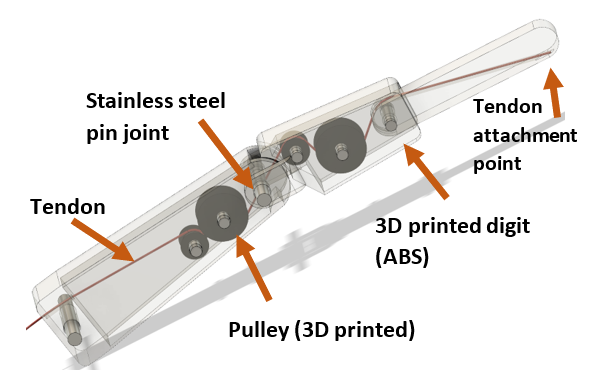
\includegraphics[width=\textwidth]{pulley} \label{pulleysys}
    \caption{Pulley system.}
  \end{minipage}
  \hfill
  \begin{minipage}[b]{0.2\textwidth}
    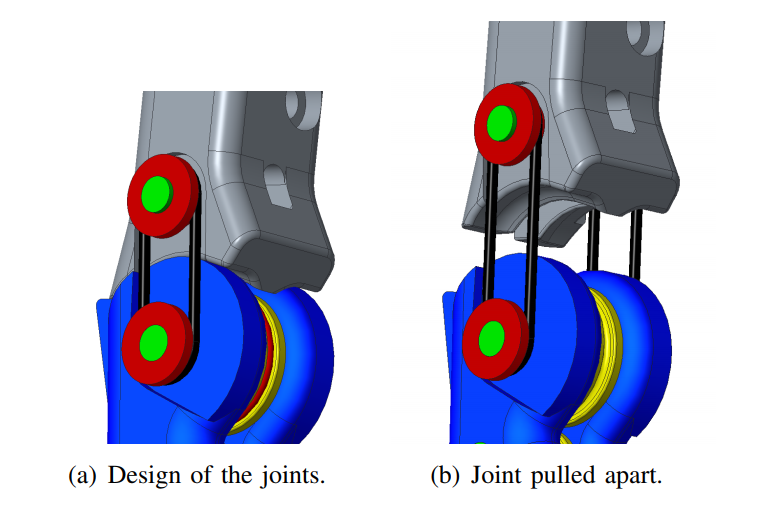
\includegraphics[width=\textwidth]{Elasticjoint} \label{eljoint}
    \caption{Elastic joints.}
  \end{minipage}
  \hfill
  \begin{minipage}[b]{0.2\textwidth}
    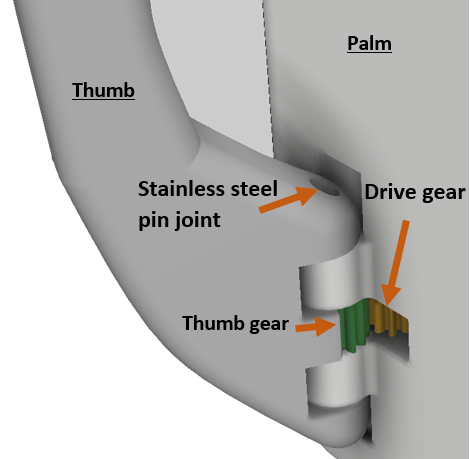
\includegraphics[width=\textwidth]{Driven_thumb} \label{dthumb}
    \caption{Driven thumb.}
  \end{minipage}
  \hfill
  \begin{minipage}[b]{0.2\textwidth}
    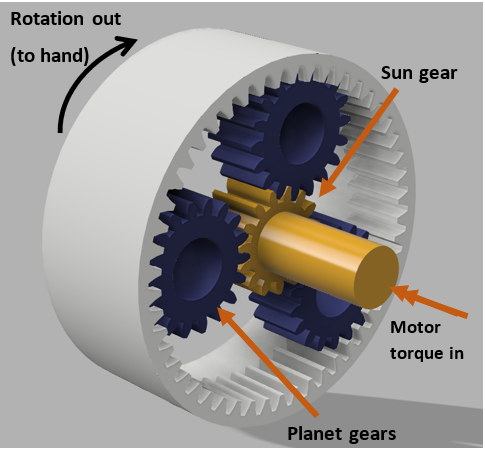
\includegraphics[width=\textwidth]{planet} \label{planet}
    \caption{Planetary gearbox.}
  \end{minipage}
\end{figure}
\normalsize

\newpage
\appendix

\bibliographystyle{plain}
\bibliography{proj}

\end{document}
